\documentclass{article}
\usepackage[utf8]{inputenc}
\usepackage{biblatex}
\usepackage{graphicx}
\usepackage{float}
\usepackage[left=1in,top=1in,right=1in,bottom=1in,nohead]{geometry}
\usepackage{enumitem}
\usepackage[colorlinks]{hyperref}
\hypersetup{
    urlcolor=blue,
    }
\addbibresource{./citations.bib}


\newcommand{\fref}[2][]{%
  \ifthenelse{\equal{#1}{}}%
	{Fig.~\ref{fig:#2}}%
	{Figure~\ref{fig:#2}}}

%================================================================================
% main document
\title{Rubik's Cube Solver}
\author{HMC SciComp Final Project}
\date{Adam Walker, \t May 7, 2021}

\begin{document}
\maketitle

%========================================
\section{Introduction}

A Rubik's Cube is a cubic 3D puzzle where turns change the locations of various stickers on the puzzle. The original 3x3x3 puzzle consists of six faces, each with nine stickers arranged in a three by three grid. The object is to solve a scrambled puzzle such that all stickers on a given face are the same color.

A Rubik's cube solver takes as input a state of the puzzle, and as output returns a sequence of moves that, when performed, put the puzzle into a solved state.

A variety of solutions have been developed to solve a Rubik's Cube. Some methods are better for speedsolving, in which a human tries to solve the puzzle as quickly as possible \cite{speedcubing}. However, in this paper, we explore computational methods that rely on modified brute forcing techniques to generate close-to-optimal solutions.

Computer-based solving approaches have numerous implications for the speedsolving community. For example, computer solvers have been used in recent years to generate new algorithms (sequences of moves that affect a particular subset of pieces in a particular way) for speedsolvers. In addition, solutions generated by computerized solvers are the backbone of generating sequences of moves to scramble Rubik's cubes. This is important for modern speedsolving competitions, which rely on scrambling programs to ensure that all competitors are given puzzles that are comparable in difficulty \cite{wca-scrambles}.

% Modern scrambling programs rely on generating a random scramble state (i.e. one state is chosen out of all possible Rubik's cube states, where every state has an equal probability of being chosen). Then, a solving algorithm is used to determine how to solve the puzzle from that state. Finally, we can invert the solution that the solving algorithm generates, providing us a sequence of moves that takes us from a solved state to the random scrambled state. For official competitions, the World Cube Association, which governs speedsolving competitions worldwide, uses this exact approach to generate scrambles.

In this paper, we discuss a variety of techniques used in computerized solving algorithms. Then, based on other existing algorithms, we develop a 3x3x3 Rubik's Cube solver in Python. Finally, we compare the results of this solver to other, more established solvers and discuss possible improvements.

\section{Existing Computer Algorithms}

We now examine existing algorithms used to solve Rubik's cubes.

We begin by examining a naive, brute foce algorithm. This algorithm hypothetically attempts every possible sequence of moves to reach every possible state, hoping to eventually find a solution. Note that the runtime of this algorithm scales exponentially. Naively, there are $6$ possible faces that can be turned, and each face can be turned one of $3$ ways (clockwise 90 degrees, counterclockwise 90 degrees, or 180 degrees). Therefore, such an algorithm scales as $O(18^n)$, where $n$ is the number of moves. While there are ways to decrease the base of $18$ (for example, by ensuring we don't perform the same move twice in a row), this naive algorithm is still intractable in the general case of a 3x3x3 puzzle.

Existing algorithms overcome these runtime issues primarily in one of two ways: either by using a heuristic-based approach for choosing moves, or by using a multi-phase approach.

One heuristic-based approach is Korf's algorithm \cite{korf}. Similar to the brute force algorithm described earlier, it examines every possible move. However, it uses a heuristic to estimate how far away a particular state is from being solved. In this way, the algorithm prioritizes performing moves that get closer to a solved state. 
% For example, one possible heuristic is to examine how far just the $8$ corners are from being solved. Since examining this subproblem is much more tractable for a modern computer (for example, on the scale of $10^7$ possible states, as opposed to $4.3*10^19$) the corresponding values can be evaluated and stored in a lookup table ahead of time for quickly evaluting the heuristic for a particular puzzle state.

An alternative approach is to use a multi-phase approach. In this approach, instead of attempting to solve directly from a scrambled state to a solved state, the solver attempts to go from a scrambled state to some new state with a particular property (for example, corners positioned in a particular way). From this state, the solver might then go to a further restrictive second state. This process continues until brute forcing to a solved state becomes tractable.

Two existing algorithms use this multi-phase approach: Thistlethwaite's algorithm and Kociemba's algorithm. Thistlethwaite's algorithm performs four stages \cite{thistle}, and the newer Kociemba's algorithm combines pairs of stages from Thistlethwaite's algorithm to create a two-stage algorithm \cite{kociemba-2phase}. The solver described in this paper will use a three-phase algorithm similar to these approaches. % We will implement a two-stage approach comparable to Kociemba's algorithm to solve a 2x2x2, and then explore a three-stage approach for solving 3x3x3 puzzles.


%========================================
\section{Definitions}

\subsection{Moves}
On a standard 3x3x3 Rubik's cube, there are $6$ centers (pieces with a single sticker) in the middle of each face. In addition, there are $12$ edge pieces and $8$ corner pieces. An edge is a piece with $2$ stickers, whereas a corner has $3$.

We define a state of the puzzle based on both the permutation (whether pieces are switched in position) and orientation (whether an individual piece is flipped) of corners and edges. Note that we define state relative to fixed centers; for example, rotating the entire puzzle without performing any moves does not change the state of the puzzle.

We can perform a variety of turns on a puzzle. Our solver denotes these turns according to the Outer Block Turn Metric \cite{wca-regs}. Relative to a solver holding a puzzle, there are six possible faces we can turn: Right, Left, Up, Down, Front, and Back. We denote these faces with the letters $R$, $L$, $U$, $D$, $F$, and $B$, respectively. For each face, there are three possible directions we can turn: clockwise by 90 degrees, counterclockwise by 90 degrees, and 180 degrees. We append an apostrophe ($'$) or a numeral two ($2$) to a given face's letter to represent turning counterclockwise or 180 degrees, respectively. For example, the sequence $R\ U\ R'\ U2$ corresponds to moving the (R)ight face clockwise, then the (U)p face $90 \deg$ clockwise, then the (R)ight face $90 \deg$ counterclockwise, and finally the (U)p face $180 \deg$.

% \subsection{Tree Representation}

% It is useful to examine states of a Rubik's cube in the context of a tree. In this representation, nodes of the tree represent states of the puzzle, and an edge between two nodes represents a move performed to get from the state represented by the parent node to the state represented by the child.

% For example, suppose we let the root node (depth $0$) be a solved 3x3x3 puzzle. From the solved state, we can perform one of $18$ possible moves ($6$ faces, times $3$ possible directions), resulting in $18$ states that are one move away from being solved. Therefore, we create $18$ nodes at a depth of $1$, and draw edges labeled with a corresponding move from the root node to each of these $18$ children. For each of these children, we can perform one of $18$ possible moves again, resulting in $18^2$ nodes at the depth of $2$. If we continued this process long enough, we'd recover every possible state, and possible solutions for a particular state are represented by paths from the corresponding node to the root node in the tree.


% The branching factor on a 2x2x2 puzzle is defined similarly. However, note that there exists a symmetry: without loss of generality, the move $R$ on a 2x2x2 is equivalent to the move $L$, in that the corner orientation is the same. Therefore, we can represent all possible moves on a 2x2x2 using only three faces instead of six, resulting in a branching factor of $9$ ($3$ faces, times $3$ possible directions).

We define the branching factor to be the number of possible moves that can be performed from a particular state. In general for a 3x3x3, the branching factor is $6 \times 3 = 18$, since we can turn $6$ faces in $3$ possible ways.

Given every possible state for a puzzle, there exists some state that takes the greatest number of moves to solve optimally. We define God's number as this number of moves. For a standard 3x3x3 puzzle, God's number is $20$ \cite{god}. 

These numbers help shed light on why naively brute forcing is so intractable: the branching factor of $18$, combined with God's number of $20$, mean upwards of $O(18^{20})$ cube states to iterate through.

\subsection{Group Theory}

Finally, we define ways of creating sets of states that contain certain properties. One method of doing this is by examining which moves are required to solve the puzzle, which we denote using a bracket notation.

By default, we denote the group of all states as $\langle R, U, F, L, D, B \rangle$. This notation signifies the set of states that can be solved using some sequence of 90 degree turns on any face. (Note that "90 degree turns" also include 180 degree and 270 degree turns, which are two or three 90 degree turns in a row). In other words, states in the group $\langle R, U, F, L, D, B \rangle$ can be solved using any of the $18$ possible moves: R, R', R2, U, U', U2, F, F', F2, L, L', L2, D, D', D2, B, B', B2.

We can create more restrictive groups that decrease the number of possible moves. For example, the group $\langle R, U, F2, L, D, B2 \rangle$ is the set of states that can be solved using only 180 degree turns on the front and back faces, and 90 degree turns on any other face. Therefore, this group reduces our branching factor from $18$ to $14$, since F, F', B, and B' are disallowed moves in this group. This aides in brute forcing solutions faster, since decreasing the branching factor makes the base of our exponential runtime lower.

% For the implementation of a 2x2x2 solver, we can define the following groups:
% \begin{itemize}
%     \item $G0 = \langle R, U, F \rangle$, the set of all scrambled 2x2x2 puzzles,,
%     \item $G1 = \langle R2, U, F2 \rangle$, the set of 2x2x2 states where the corners are oriented with respect to the up and down faces (i.e. the up and down face stickers only include stickers from the up and down faces), and
%     \item $G2 = \langle  \rangle$, the solved state.
% \end{itemize}

For the implementation of a 3x3x3 solver, we define the following groups:

\begin{itemize}
    \item $G0 = \langle R, U, F, L, D, B \rangle$, the set all 3x3x3 states;
    \item $G1 = \langle R, U, F2, L, D, B2 \rangle$, the states with edges "oriented" relative to the front and back faces \cite{eo};
    \item $G2 = \langle R2, U, F2, L2, D, B2 \rangle$, which corresponds to states with all edges oriented, plus all up and down face stickers on the up and down faces. This is commonly known as a "Domino" reduction \cite{domino}; and 
    \item $G3 = \langle 1 \rangle$, the set containing the single solved state.
\end{itemize}

%========================================

\section{Solver Implementation}

Each phase of a multi-phase algorithm attempts to find a short sequence of moves to go from some group $G_n$ to another group $G_{n+1}$, using only the moves allowed for that group. For example, in the final step of the 3x3x3 solver, the program takes as input a puzzle in a G2 state, and brute forces combinations of $\langle R2, U, F2, L2, D, B2 \rangle$ moves (R2, U, U', U2, F2, L2, D, D', D2, and B2) to solve the puzzle. Since each successive group becomes more and more restrictive in terms of which moves can be performed, the branching factor decreases with successive phases, leading to a more tractable runtime.

We can also employ a variety of additional techniques to make runtime even faster.

\subsection{Table Lookup}

In many circumstances, we can enumerate many of the possible states ahead of time. For example, given a solved 3x3x3, we can enumerate out all possible states that are within $m$ moves of being solved. Then, for each possible state we enumerate, we create an entry in a hash table, where the key is a hashed state of the puzzle and the value is a breadcrumb that allows for recovering a solution of length $\leq m$.

Performing this precomputation can have a dramatic effect on runtime. For example, suppose we have a puzzle in a "Domino" (G2) state, as described earlier, and we wish to compute a solution to the puzzle from that state. The median domino state takes $13$ moves to solve, and domino reductions have a branching factor of $10$. Thus, naive brute forcing requires approximately $10^{13}$ iterations. However, if we create a table ahead of time with $m=8$, we now only have to brute force into any state that is within $8$ moves of being solved, since recovering the remaining $8$ moves becomes trivial. Thus, instead of brute forcing $10^{13}$ iterations, we can brute force $10^{13-m} = 10^5$ iterations.

Unsurprisingly, generating these tables is exponential in runtime. For generating the domino table described previously with $m=7$, my single-threaded implementation took approximately two hours. For $m=8$, I ran the table generator overnight.

\subsection{Preventing Repeated Moves}

Another improvement is to ensure moves are not repeated. For example, suppose when brute forcing that we just performed the move $U$ (up face clockwise). We can remove $U'$ (up face counterclockwise) from consideration, since we would be undoing the progress we just made. Similarly, without loss of generality, we wish to ignore sequences like $R$ followed by $R2$, since a 270 degree clockwise turn ($R\ R2$) is equivalent to a 90 degree counterclockwise turn ($R'$). These adjustments further reduce our branching factor.

\subsection{Using Previous Solutions as an Upper-Bound}

As the program continues to run, it seeks strictly shorter and shorter solutions, which we can use to bound how long later steps run. For example, suppose our program is running and has already found a solution of length 35. Then, let's suppose it is considering a new sequence of moves that takes us from the scrambled state to a G2 state in $28$ moves. Since we now only wish to consider overall solutions that are strictly less than 35 moves in length, we know this 28-move candidate is only valid if we can solve the remainder of the puzzle (G2 to G3) in less than $35-28 = 7$ moves. Thus, for the last step, we can force our program to stop running and instead consider other candidates once it has brute-forced every sequence that is less than $7$ moves.

Note that our implementation combines many of these techniques. For instance, suppose we force the last step to stop after $7$ moves like the above example, and our lookup table for the last step stores all states that are within $8$ moves of being solved. To determine if a solution of less than $7$ moves exists, our last step merely has to check if an entry exists in the table. This can be done in $O(1)$ time.

%========================================

\section{Implementation}

Our three-phase 3x3x3 solver is written in Python. Note that we use Ramon Griffo's library \cite{git-lib} to represent a 3x3x3 puzzle. This library provides a data structure to store the puzzle, supports making turns on the puzzle, and has additional helper methods, such as determining if a puzzle is solved or printing the puzzle to a console window.

\subsection{Code}

The full code implementation is available on Github \cite{git-solver}.

The repository contains a 2x2x2 solver used as a proof of concept, in the form of an interactive Jupyter notebook. It contains a brute force implementation, and then develops a two-phase approach to solving a 2x2x2.

The 3x3x3 solver is broken up multiple files that are each responsible for solving a particular phase. \emph{eo\_solver.py} solves from G0 (scramble) to G1 (edges oriented). Then, \emph{eq\_solver.py} takes as input a cube in G1 and outputs a different cube in a subset of G1 where all edges in the up and down faces contain stickers from the up or down face. This allows \emph{co\_solver.py} to then solve to a G2 state. Finally, \emph{domino\_solver.py} solves from a G2 to a solved (G3) state. \emph{gen\_domino\_table.py} generates a lookup table, which is stored locally as a Pickle file and is used by \emph{domino\_solver.py}. 

\emph{overall\_solver.py} performs each step sequentially, and samples multiple possible solutions at each stage. For example, the solver may have \emph{eo\_solver.py} generate multiple ways of getting to a G1 state. Then, given a particular way of solving to G1, the solver attempts to find a way of solving the rest of the puzzle. In this way, the solver may find less optimal solutions quickly but closer to optimal solutions as it continues running and sampling different possibilities at each stage.

%========================================
\begin{figure}
	\centering
    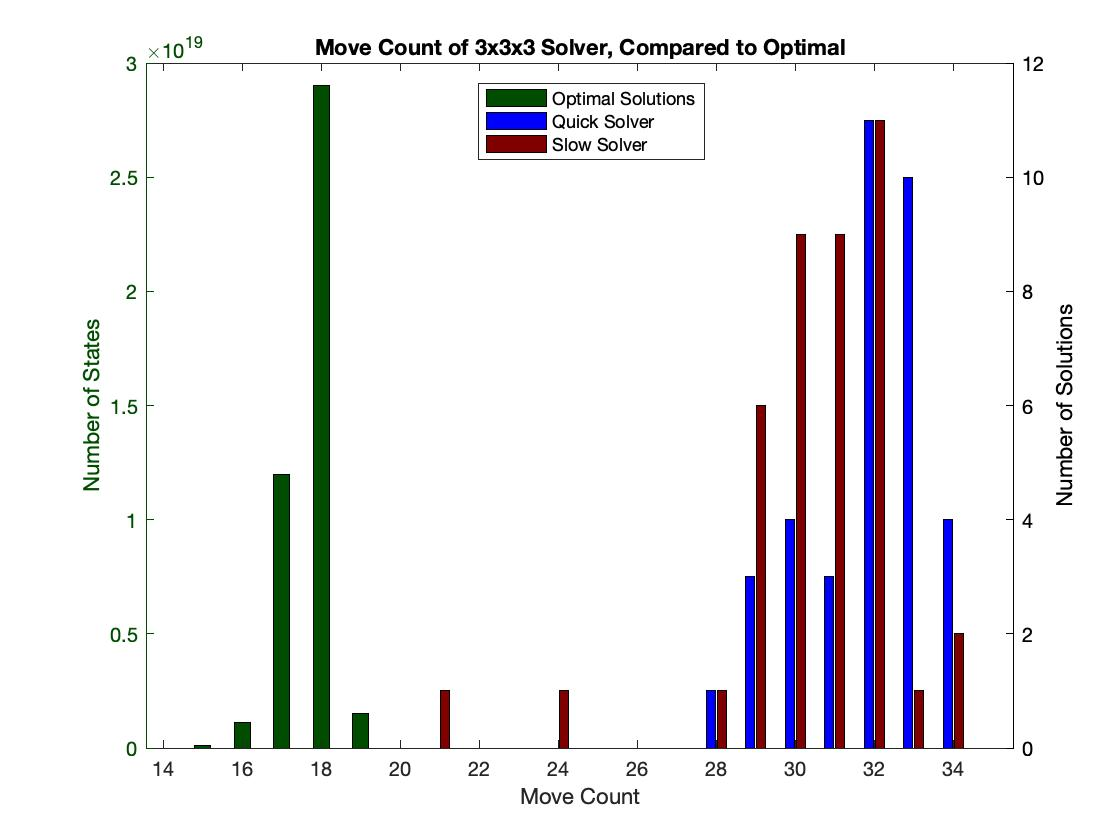
\includegraphics[width=5in]{movecount.jpg}
	\caption{We run the 3x3x3 solver for $42$ trials using two sets of parameters. The "quick" solver (blue) only looks for $2$ solutions from G0 to G1 states. For each possible solution, the solver then attempts to find solutions for the remainder of the puzzle (from G1 to solved), and returns the better of the two. The "slow" solver (red) instead finds $15$ possible solutions from G0 to G1 and tests each of the $15$, at the expense of running time. We can compare this distribution to the lengths of optimal solutions (green). For each of the $43$ quintillion states, there exists some optimal solution with length between $1$ move and $20$ moves; we plot number of states with each length, the vast majority of which fall between 16 and 19 moves \cite{god}. Due to the parameters set in later stages of the algorithm, the quick solver failed to find solutions for $6$ out of the $42$ scrambles, and the slow solver failed to solve $1$ scramble.}
	\label{fig:movecount}
\end{figure}
\section{Results}

To test the implementation, we generate $42$ random scrambled states of the puzzle \cite{cstimer}. Then, for each scramble, we perform two runs of our solver: a slow run and a quick run. The slow run finds $15$ solutions to the first step (G0 to G1). For each of the $15$ possibilities, it then attempts to find solutions to the remainder of the puzzle, progressively finding better solutions over time. The quick run reduces this number from $15$ to $2$, which results in faster runtime for both the G0 to G1 step and fewer computations for the remainder of the puzzle.


The solver was run on a MacBook Pro with a 6-core 2.6 GHz processor and 16GB of RAM. Since the solver only takes advantage of a single core and uses less than $3$GB of RAM, five instances of the solver were run at any given time.

The quick solver took a median time of $9.05$ minutes (min: $2.78$ minutes, max: $140.5$ minutes). \fref{runtime} shows the runtime for each quick run. Unfortunately, the runtimes for the slow runs were lost; however, the slow runs took a total of approximately $36$ hours total to run.

\begin{figure}
	\centering
    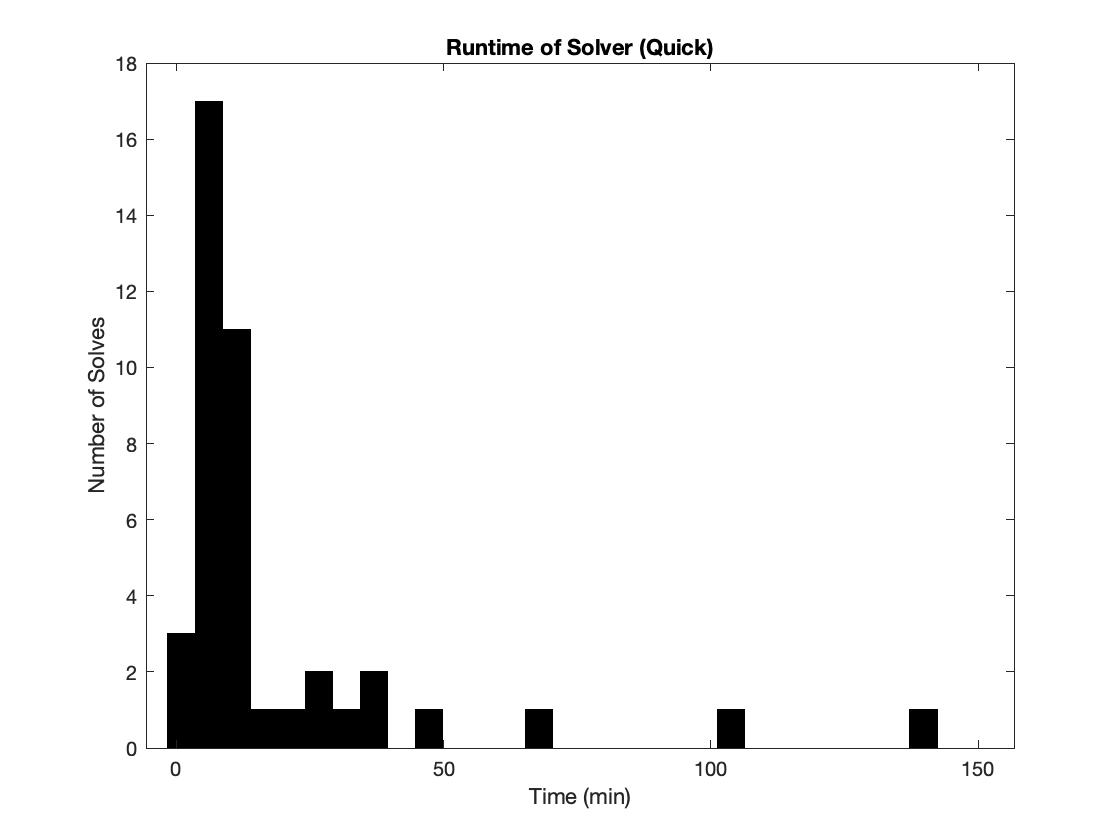
\includegraphics[width=6in]{runtime.jpg}
	\caption{Runtime of solver for 42 trials, using the "quick" parameter set (only finding $2$ solutions from G0 to G1). A vast majority of solutions were found in less than a half hour.}
	\label{fig:runtime}
\end{figure}

The quick solver's solutions averaged 31.8 moves (min: 28, max: 34), and the slow solver averaged 30.5 moves (min: 21, max: 34). \fref{movecount} compares the move counts for both the quick and slow runs. This figure also displays the distribution of the optimal solutions for all $43$ quintillion Rubik's Cube states \cite{god}. Out of all possible states, the vast majority are solved optimally in either $17$ or $18$ moves. Therefore, our solver in these $42$ trials found solutions that are approximately twice optimal in length. 

We can compare these results to existing multi-phase algorithms. Kociemba's algorithm, which uses two phases instead of three, solves every puzzle in a maximum of $23$ moves and in a median of $18$ moves \cite{kociemba-dist}. Thistlethwaite's algorithm, which uses four phases, solves in an average of $31$ moves \cite{thistle-dist}. Though my solver uses three phases, there are many limitations (discussed below) that result in earlier phases (from G0 to G2) being suboptimal. For comparison, Kociemba's algorithm solves from G0 to G2 optimally in a single step. Note that our implementation always solves the last step (G2 to G3) optimally, like Kociemba's algorithm.

Note that the numbers of $2$ and $15$ for quick and slow runs were chosen as proxies for determining how running longer affects solution length. It is possible to choose even higher numbers in order to find better solutions, at the expense of runtime. Similarly, we could also tweak parameters of other phases of the solver, which were kept fixed in these trials in a manner that balances runtime and solution length.


%========================================

\section{Limitations and Future Work}

There are a variety of limitations in the implementation described above that result in the algorithm being suboptimal, both in terms of runtime and in terms of the length of the solutions generated. % There are a variety of features in more established solvers, such as Cube Explorer, that are lacking here.

\subsection{Platform Limitations}
The solver is implemented using Python, and even simple operations like simulating the turning of a face require switching multiple entries within a NumPy array. Better optimized solvers typically use lower-level languages, such as C or C++, and rely on bitwise operations that perform these types of operations more efficiently \cite{kociemba-coord}.

\subsection{Symmetry Arguments}
The implementation above does not take into account the symmetry of different states of the puzzle. One example of this is that the algorithm arbitrarily chooses the face with the white center as the "up" face, and solves into the groups G1 and G2 relative to this choice. We could just as easily define any other face (say, the face with the red center) as the "up" face, which could lead to shorter solutions.

\subsection{Using Heuristics for Searching}
All brute-forced steps in our implementation rely on a traditional breadth-first search. In contrast, recall that Korf's algorithm uses heuristics to prioritize performing certain moves that lead closer to a solved state.

We could apply a similar idea to our algorithm. This would involve replacing the breadth-first search currently used for brute-forcing with a heuristic-based depth-first search algorithm, such as Iterative Deepening A* \cite{ida}. This would also require generating lookup tables for the values of those heuristics, based on particular corner or edge properties.

\section{Conclusion}
In this project, we implemented a 3x3x3 Rubik's cube solver based on existing algorithms and techniques. The solver takes on the scale of minutes to generate solutions that are approximately twice optimal in length.

While this solver does not perform as well as other existing implementations, this implementation sheds light on many of the techniques that those solvers employ as they grapple with something that is inherently exponential in runtime.

\section{Bibliography}
\printbibliography[heading=none]


%========================================
\end{document}